\chapter{Description de la solution}
\section{Mise en cadre du projet\label{cahiercharges}}
Rappelons que la solution doit :
\begin{enumerate}
  \item assurer suivi de l'activité cardiaque,
  \item effectuer sauvegarde des différentes valeurs,
  \item la base de donnée doit être accessible via le web.
\end{enumerate}
\section{Composante matérielle}
En se basant sur les recommendations de la section \ref{cahiercharges}, la selection des équippements peut être raffinée. Comment peut effectuer le suivi de l'activité cardiaque? l'un des capteur permettant une telle opération est le capteur AD8232. La section suivante donne plus de détails.
\subsection{Le capteur AD8232 \label{sec:capteurAD8232}}
Le module AD8232 assure la surveillance des impulsions cardiaque. Le kit apporte en plus 3 électrodes à placer sur le corp du patient. Ce module, dont le datasheet est disponible sur ce \href{https://www.analog.com/media/en/technical-documentation/data-sheets/ad8232.pdf}{lien} (voir Annexe \ref{Datasheet}), est caractérisé principalement par :
\begin{itemize}
  \item un filtre passe-haut à deux pôles pour éliminer les artefacts de mouvement et le potentiel de demi-cellule d'électrode
  \item un amplificateur opérationnel sans contrainte pour construire un filtre passe-bas à trois pôles éliminant les bruits suplémentaires
  \item température nominale de $[0;70]$ et de travail $[-40; 85]$
  \item alimentation faible de 3,3V
  \item il est conçu pour extraire, amplifier et filtrer les petits signaux bipotentiels en présence de conditions bruyantes.
\end{itemize}

\begin{figure}[H]
  \centering
  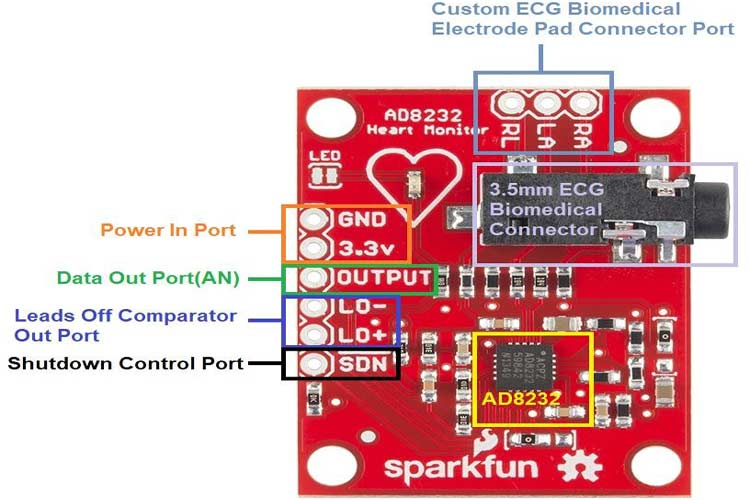
\includegraphics[scale=.4]{imgs/AD8232-Module-Overview.jpg}
  \caption{Description du capteur AD8232}
\end{figure}

Le tableau \ref{table:AD8232PINOUT} donne les pins du capteur
\begin{table}[H]
  \centering\small
  \begin{tabular}{lp{0.6\textwidth}}
  \toprule
  {\bf PIN}&{\bf Description}\\
  \toprule
  \mintinline{c++}{GND}&la masse\\
  \midrule
  \mintinline{c++}{3.3V}&alimentation\\
  \midrule
  \mintinline{c++}{Output} (ADC)&la sortie traitée du signal\\
  \midrule
  \mintinline{c++}{LO-}&leads off detection mode. \mintinline{c++}{LO-} est \mintinline{c++}{HIGH} si l'électrode rouge est déconnectée, et \mintinline{c++}{LOW} sinon\\
  \midrule
  \mintinline{c++}{LO+}&leads off detection mode. \mintinline{c++}{LO+} est \mintinline{c++}{HIGH} si l'électrode jaune est déconnectée, et \mintinline{c++}{LOW} sinon\\
  \midrule
  \mintinline{c++}{SDN}&Shutdown Control Input. Si cette pin est \mintinline{c++}{LOW}, le capteur active le mode de faible consommation\\
  \bottomrule
  \end{tabular}
  \caption{AD8232 PINOUT}
  \label{table:AD8232PINOUT}
\end{table}
\subsection{Carte de développement}
La section \ref{sec:capteurAD8232} a détaillé les carectéristiques techniques du capteur. Maintenant, une foi le capteur délivre l'activité électrique via sa pin \mintinline{c++}{Output}, vers quelle carte de développement cette information sera finalement acheminée ?

Pour répondre à cette question, il est recommander de revoir les recommendations citées dans la section \ref{cahiercharges}. En effet, l'activité cardiaque doit être envoyée vers le WEB. Ce qui impose que la carte doit pouvoir se connecter à INTERNET. Une recherche comparative entre les différents boards éligibles tels que Arduino (avec ses variantes), STM32, ESP32 \ldots a été établie. Les critères de sélection retenus sont la connectivité, le prix et la disponibilité. Finalement, la carte ESP32 est celle qui répond mieux aux différentes contraintes. Elle offre plusieurs types de connectivités (WIFI, Bluetooth) avec un prix minimal.


\begin{figure}[H]
  \centering
  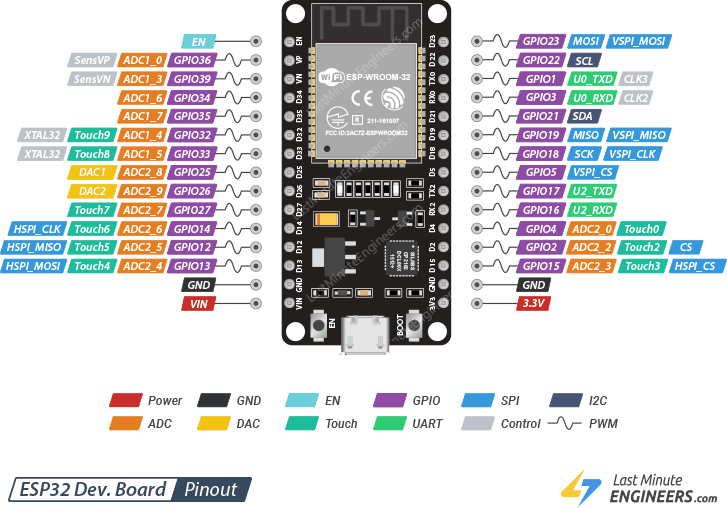
\includegraphics[scale=2]{imgs/ESP32-Pinout.png}
  \caption{Description de la carte de développement ESP32}
\end{figure}

L'ESP32 est un microcontroleur dont le constructeur est \textit{Espressif}. Ce constructeur a développé tout un système temps réel (FreeRTOS) pour ce microcontroleur. C'est pourquoi il est bien adapté aux applications temps réel et IoT. Il est caractérisé principalement par :
\begin{itemize}
  \item CPU : Xtensa double-cœur (ou simple-cœur), microprocesseur LX 32 bits, fonctionnant à 160 ou 240 MHz et fournissant jusqu'à 600 DMIPS, avec un
  coprocesseur ultra basse consommation (ULP)
  \item Mémoire : 520 KiO SRAM
  \item Connectivité sans-fil : Wi-Fi : 802.11 b/g/n;
  Bluetooth : v 4.2 BR/EDR et BLE jusqu'à v 5.0 et v 5.1
  \item 10 $\times$ capteurs de touché
  \item 4 $\times$ SPI
  \item 2 $\times$ interfaces I²S
  \item 2 $\times$ interfaces I²C
  \item 3 $\times$ UART
  \item interface MAC Ethernet avec DMA dédié et support du protocole de temps précis IEEE 1588
  \item Bus de données CAN 2.0
  \item Moteur PWM
\end{itemize}
\subsection{Assemblage}
La connection du capteur AD8232 avec la carte ESP32 doit suivre le schéma suivant :

\begin{figure}[H]
  \centering
  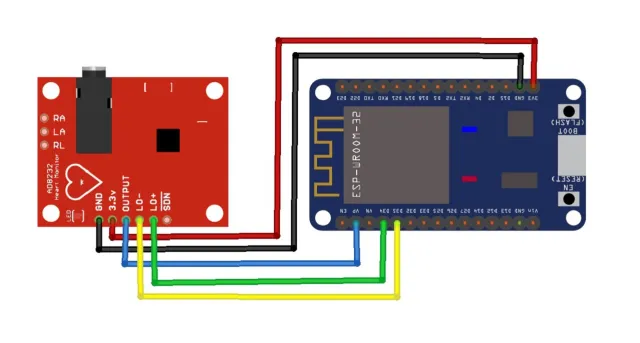
\includegraphics[scale=.4]{imgs/AD8232ESP32.png}
  \caption{Interfaçage du capteur AD8232 avec la carte de développement ESP32}
\end{figure}

Pour que le système soit en marche, il faut ajouter :
\begin{enumerate}
  \item une connexion INTERNET : la carte ESP32 peut se connecter à un réseau WIFI. Mais un tel réseau doit assurer une connexion à INTERNET et n'est pas un simple réseau local par exemple.
  \item un serveur de données : il faut avoir un accès à un serveur dans le WEB afin d'y enregistrer les informations récupérées du capteur. Ainsi, une inscription dans une plateforme dédiée peut donner ce type d'accès.
\end{enumerate}

Jusqu'à présent, la partie hardware du projet a été investiguée. En se basant sur cette architecture, quels sont les composants software à ajouter permettant le bon fonctionnement du système ?
\section{Composante logicielle}